\section{Background}
\label{sec:background}

\subsection{RDMA}

\todo{this section needs to be crunched down}

\begin{figure*}[t]
    \centering
    \begin{subfigure}{0.3\linewidth}
        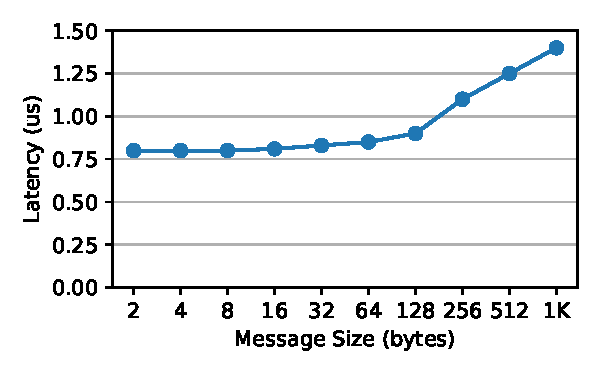
\includegraphics[width=0.99\linewidth]{fig/rdma_latency.pdf}
        % \label{fig:rdma_latency}
        % \caption{}
    \end{subfigure}
    \begin{subfigure}{0.3\linewidth}
        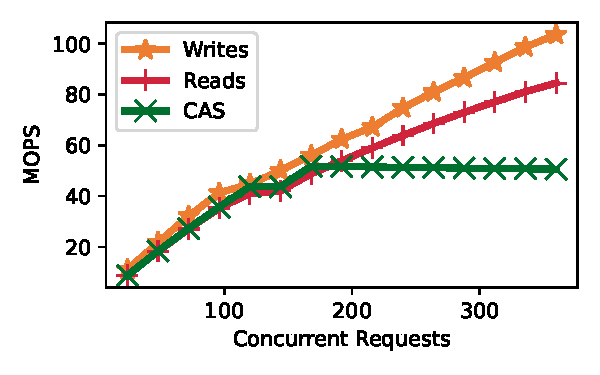
\includegraphics[width=0.99\linewidth]{fig/rdma_concur.pdf}
        % \label{fig:optimistic_failures}
        % \caption{}
    \end{subfigure}
    \begin{subfigure}{0.3\linewidth}
        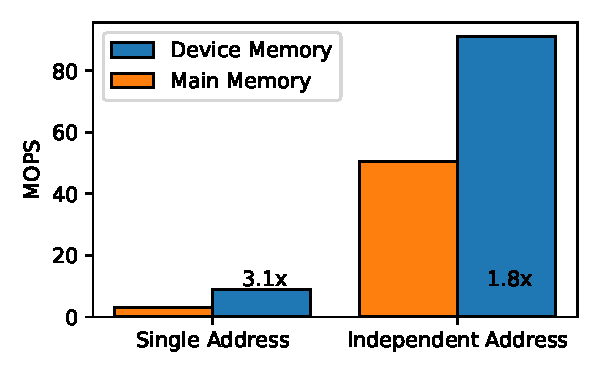
\includegraphics[width=0.99\linewidth]{fig/rdma_cas_throughput.pdf}
        % \label{fig:optimistic_failures}
        % \caption{}
    \end{subfigure}
    \vspace{-1em}
    \caption{
    \textbf{(a)} CX5 RDMA latency vs message size~\cite{rdma-latency}
    \textbf{(b)} RDMA operation scalability
    \textbf{(c)} Compare and swap performance. Device memory vs main memory.
    }
    \label{fig:rdma-benchmarks}
\end{figure*}

RDMA is an enabling technology for memory disaggregation. It
allows client machines to directly access the memory of a
remote server with operations like read, write and atomic
update, without the involvement of a remote CPU (save for
initialization).  
%%
In the past decade the bandwidth
capabilities of RDMA NICs have increased disproportionately
to their latency improvement. The bandwidth difference
between CX3 and CX7 NICs is 10$\times$ and yet intra-rack
round trips of small RDMA packets has only shrunk by around
1.5$\times$.  Figure~\ref{fig:rdma-benchmarks}(a) shows the
tradeoff between NIC-to-NIC round trips times on CX5 RDMA
NICs for write operations. All packets up to 128 bytes have
comparable round trip latencies, and packet sizes must grow
to above 1K before the latency cost of a large packet
exceeds the cost of two round trips for smaller packets.
\textbf{If there is surplus bandwidth a single large message
can have much lower latency than two dependent smaller
messages}

RDMA verbs do not all have the same performance. Atomic
operations such as compare-and-swap (CAS) and fetch-and-add
(FAA) both have bottlenecks much lower than reads and
writes~\cite{design-guidelines,sherman}.
Figure~\ref{fig:rdma-benchmarks}(b) shows the scalability of
these operations on CX5 NICs for 64 bit operations.
%%
Atomic operations bottleneck due to PCIe round trips. 
Each operation issued from NIC to host memory requires a
PCIe round trip. Data dependent operations must queue until
the atomic operation completes.
%%
Vendors have recently provided a small region (256KB)
of device mapped memory which avoids the round trip on
atomic operations~\cite{device-memory}.
Figure~\ref{fig:rdma-benchmarks}(c) shows the relative
performance of CAS operation on device memory vs host
memory. Lock request on a single address are 3x higher
throughput, and independent lock requests scale at nearly
the same rate as read and write requests.

Additionally Mellanox provides non-standard verbs such as
64-bit masked compare-and-swap which sets individual bits in
a 64 bit word independently of unmasked
bits~\cite{rdma-masked-cas} This is useful for setting
multiple independent locks, assuming locks are close
together, as the state of all locks need not be known.


\subsection{RDMA Key-Value Stores}

%% %Describe existing key value stores relation to rdma and
%serialization %
Many non-disaggregated key-value stores have used RDMA to
accelerate their
performance~\cite{farm,memc3,erpc,herd,faast,mica,pilaf,cell,storm}.
%%
These systems strike a careful balance between directly
accessing memory with client side RDMA and serializing
requests with a server side CPU.
%%
Cuckoo and Hopscotch hashes have flourished in this space
because clients can locally calculate the location of keys
and perform lockless $O(1)$ reads with
RDMA~\cite{hopscotch,farm,pilaf,cuckoo}.
%%
Disaggregated key-value in contrast assume that a memory
server cannot provide serialization and orchestrate their
writes solely using
clients~\cite{rolex,fusee,clover,sherman,ford,race}. With
the exception of Sherman these systems use systems commit
writes optimistically using 64 bit RDMA CAS. 
%%
Opportunistic writes have the advantage that updates are
atomically visible, no critical sections exist, and client
failures do not leave the table in an inconsistent state.
However, opportunistic concurrency comes at a cost.
Contention leads to frequently failed operations and high
tail latencies~\cite{clover}, CAS operations don't scale
well~\cite{design-guidelines}(Figure~\ref{fig:rdma-benchmarks}(b))
and 64 bit width CAS constrain the size of updates to the
table.

CAS width in particular effects system design.  Because
key-value pairs can rarely fit into 64 bits, indexes updated
with CAS must reference keys values indirectly with a
pointer. At minimum resolving a remote pointer requires an
additional round trip for every read~\cite{race,clover}.
%%
As we will show in the following section data structures
like cuckoo and hopscotch hashes are difficult implement with
optimistic CAS updates because they require multiple updates
to execute atomically.


\subsection{Cuckoo Hashing} 

Cuckoo hashing uses two independent hash functions to give
keys a primary and secondary location in the table. When an
insert collides with an existing key, the existing key is
evicted to its alternate location. If the eviction also
causes a collision the process iterates. The path of
evictions is known as a~\textit{cuckoo path}. Cuckoo hashes
use associative rows to improve fill factors. In associative
hashes multiple clients can be chosen as eviction candidates
and breadth-first-search (BFS) has been shown to minimize
both path length and critical section time~\cite{memc3,
cuckoo-improvements}. While insertions require large
critical sections to perform search and execute updates
along the cuckoo path reads are executed in constant time by
reading both of a keys buckets~\cite{pilaf}.

%%now I want to explain why cuckoo hashing and disaggregation don't work well together.

Fast parallel reads make Cuckoo hashing a desireable
candidate for a disaggregated index, however, long
unpredictable cuckoo paths and RDMA CAS limitations make
insertions difficult in the disaggregated setting. We
designed an RDMA based cuckoo hash to illustrate the
difficulties of performing opportunistic insertions. On
inserts this system makes a sequence of reads to calculate a
valid cuckoo path and then itteratitivly issues CAS
operations to swap value along the path. If any value on the
path is concurrently modified by another client the
insertions will fail and must restart.
Figure~\ref{fig:cuckoo-problems}(a) shows how the failure
rate of insertions filling a table from 80-90\% full.


% Cuckoo hashing Uses two hash functions as a means
% to resolve collisions when entries hash to the same
% location. Because entries have at most two locations, cuckoo
% hashing has constant time reads as only two locations need
% be checked to determine an entries existence, or location.
% Cuckoo tables use row associative to improve their maximum
% fill factor. Each hash location can house up to $n$
% associated elements. When locating an entry all entries in
% the row must be read.  Cuckoo inserts use the first hash
% functions location as an entry's insert row. If the row is
% full an element is chosen for from that row. The evicted
% element is hashed using it's second hash function, and is
% placed in it's alterative row. If the alternative row is
% also full, the process repeats. The sequence of evicted
% elements is known as a~\textit{cuckoo
% path}~\cite{cuckoo,memc3,cuckoo-improvements}. The search
% algorithm used to find a cuckoo path on an associative
% cuckoo table has a large impact on the length of the
% path~\cite{cuckoo-improvements}. When a path can not be
% found the table has reached it's max fill factor and the
% table will no longer accept new inserted entries. The table
% can be resized and rehashed to continue operation.

\textbf{Hopscotch Hashing}:
\todo{This section needs to be compacted and integrated with the other text}
\todo{Add Reno hash as a counter example for disaggregation}
is another candidate hash table
we considered for disaggregation. Hopscotch hashing uses a
hybrid if linear probing and swapping to ensure that hash
entries are within a constant bound of their original
location. Farm~\cite{farm} demonstrated that this location
bound is useful for RDMA as a single read can determine if
an entry is in the table. We believe that with effort a
highly performant hopscotch hash table could be built for
disaggregated memory. However, a few challenges prevented us
from pursuing hopscotch hashing. 
%%
Firstly, on insert hopscotch hashing must update at a
minimum two locations, the location the entry is written to,
and the bitmask in the location the entry hashes to. When
the table is full insertions cause hopscotch chains, each
hop of which requires two locks. As the state of the remote
hash table can change between reads and locking time we see
every additional modification as a barrier to predicting on
a client which entries should be locked.
%%
Second, cuckoo hash locations can be predicted easily. In a
bucket cuckoo hash the location of an entry can be
determined exactly by it's key. This enables clients to
predict which locations will need to be locked locally
without needing to read from remote memory. As entries can
take multiple locations in a hopscotch entry locks must be
course grained in order to guarantee that they will be
captured.
%%
Third, CRC coverage of hopscotch hashing is not obvious. As
we will show, a CRC for a single bucket in cuckoo hashing
can cover multiple entries as a single CRC can be calculated
per row in the table. In Hopscotch hashing the location and
spacing of CRC's is not obvious.
%%


% is a hash table which delivers
% constant-time reads. It uses two hash functions to determine
% two possible locations at which any hashed item can reside.
% When reading both locations are queried. If the item is not
% found, it is not in the table. On insert, the item is placed
% in the first location it hashes to. If that location is full
% the item in that location is evicted and kicked to it's
% second location.  This process happens iteratively for many
% items. The sequence of displaced keys on an insert is called
% a ~\textit{cuckoo-path}~\cite{cuckoo-improvements}. When a
% loop occurs in a cuckoo path the insert fails and the table
% is resized. Fill factors for cuckoo hashes can be improved
% by using associative buckets for each hash index, and
% shortening cuckoo paths by using BFS rather than radom
% search~\cite{cuckoo-improvements}. ~\todo{consider adding a
% cuckoo search figure}.